\section{Implementation}
To evaluate the approaches described in the previous chapter, concrete realization of an SDN
controller and data processing engine is needed. With Apache Flink, the data processing engine
constraint was already given. Besides that, a middleware software has to be implemented as a layer
between network and high level data engine. To achieve the project goals, a middleware has to be
implemented to connect low level network management via SDN controller and high level distribution
of the data processing tasks.

\subsection{SDN Controller}
In the open source community, there are some realizations of SDN controllers. The most popular ones
are POX/NOX, Floodlight and OpenDaylight. We use the de-facto standard OpenDaylight (ODL) as our SDN
Controller. It features good interoperability as well as scalability. It communicates via OpenFlow
with the virtual switches for routing and forwarding purposes as well as via a REST-interface with
custom programs, acting as a server providing network information on demand. 

\subsection{Requirements}
In the previous sections, two approaches have been introduced: Bottom Up and Top Down.
Implementation of the logic and algorithms relies on some requirements to the middleware software.
First, the middleware has to obtain information about the network topology and its current status.
To get information about the underlying network, a REST client is required to communicate with the
Northbound Topology API of OpenDaylight controller. Another requirement to the specification of the
middleware is realization of the scheduling approach. More specifically, it is about to implement an
algorithm of how the physical hosts (slots) are assigned to the tasks of the data processing engine.
This should be achieved in a way that the network communication between hosts is efficient and the
network resources are utilized as much as possible. The host assignment should be based on the
information about the network topology and the current status. The Top Down approach tries to
optimize the network utilization during runtime. The middleware needs to have information about the
currently executing job and its deployment (and distribution) in the network. This information is
provided by the data processing engine and should be transferred to the middleware. The middleware
has to analyze the data and optimize data flows by setting network flows through SDN controller. As
an optional requirement, a graphical representation of the current network topology and the host
assignment may be implemented. This functionality can be very useful for monitoring, controlling and
debugging of the middleware and the current job execution.

\subsection{Middleware Architecture}

\begin{figure}[h]
    \centering
    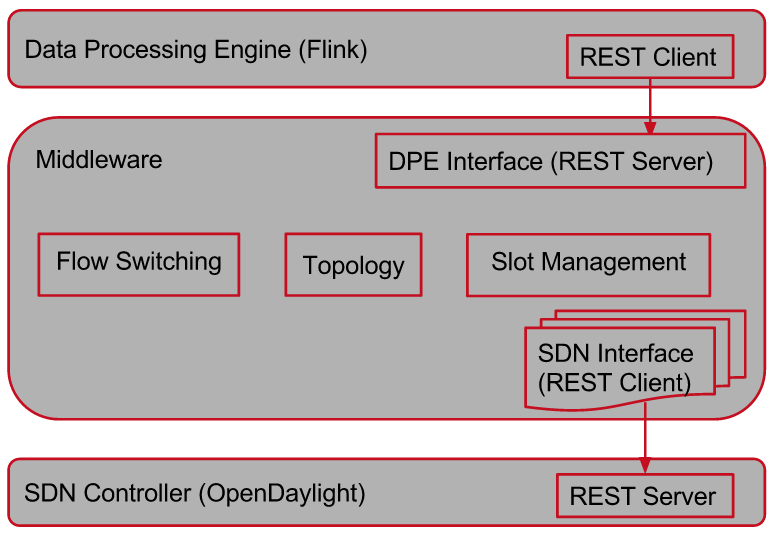
\includegraphics[width=0.8\textwidth]{graphics/architecture.png}
    \caption{Middleware Architecture}
    \label{fig:architecture}
\end{figure}

The architecture of the implemented middleware software is shown in Figure 3. The highest level in
the architecture is the data processing engine Flink. After the creation of the execution graph and
before deployment on the hosts, a communication-client has been implemented into the Flinks
scheduler-internals to communicate with the middleware. This client sends the execution graph and
requests new hosts for the job as soon as they are needed. The hosts, which finished execution are
released through a call of this client as well. The corresponding server side is a part of the
middleware. There are four other modules in the middleware. The topology module collects all the
data about the network: topology (network devices, hosts and connections between them) and the
current utilization of the network. The slot management part is responsible for slot allocation for
the distributed data engine. Algorithms behind it and the generic API belong to this module as well.
The flow switching module takes care about the optimization of the network flows based on the
current execution graph and network status. In order to access the Northbound API of the SDN
controller, generic interfaces were defined so that the middleware does not depend on one particular
implementation of a SDN controller. The concrete realization of northbound clients was done
separately for the required APIs, such as Flow Programmer and Topology API. A Module for network
visualization was implemented as well as part of the middleware. Technically, the middleware is
implemented as a Maven multi module project. This decision was made to take advantage of the
benefits of a structured project powered by a feature rich build system: flexibility,
customizability, dependency management, task automation and more. All the algorithms are covered
with tests and the source code is published under Apache License on the public repository hosting
service.

\subsection{Middleware Slot Assignment}
The I/O operations are the bottleneck of distributed data processing setups \cite{cheating}. Besides
reading and writing to disk, there is the communication layer over the network. The Bottom Up
approach should help to organize the execution slots in a way that they are able communicate in an
efficient manner over the network. In this section, the algorithm for  slot distribution over the
network is described.

\begin{figure}
    \centering
    \begin{minipage}{0.5\textwidth}
        \centering
        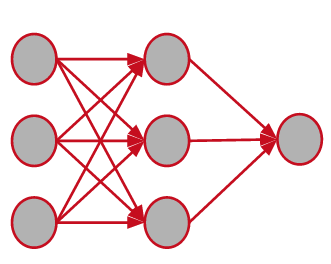
\includegraphics[width=0.6\linewidth]{graphics/executiongraph.png}
        \captionof{figure}{Execution graph}
        \label{fig:execution_graph}
    \end{minipage}%
    \begin{minipage}{0.5\textwidth}
        \centering
        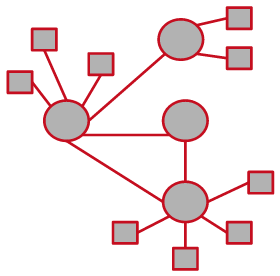
\includegraphics[width=0.6\linewidth]{graphics/topology.png}
        \captionof{figure}{Network Topology}
        \label{fig:network_topology}
    \end{minipage}
\end{figure}

As a starting point, there is the execution graph (Figure \ref{fig:execution_graph}) and the network
topology (Figure \ref{fig:network_topology}).  This information derives from data processing engine
and SDN controller respectively. Besides that, it is possible to collect data about the current
utilization of the network over the SDN controller.  The execution graph represents the steps of the
job execution and the network topology is a formation of hosts, network devices and links between
them in the network. Both of them are directed graphs. The question is how to map (apply) one graph
into another to achieve the best links between the executors.

The general approach is to find an isomorphism between the two graphs. But first, the execution
graph has to be normalized since Flink (and other data processing engines) will more likely execute
some of the nodes of execution graph on the same physical host (or even on the same slot). Because
of this, the normalization function of the graph depends strongly on the engine being used, so this
solution would be not generally applicable. Furthermore, there are no efficient algorithms available
resolving this problem (graph isomorphism problem) and even the complexity of it is
unknown.\cite{graph}

Another reasonable approach is the solution to the general heaviest k-subgraph problem. Using the
algorithms to calculate the heaviest subgraph it is possible to get k nodes of the graph which
connections have the biggest weight. Data processing engine’s deployments of the tasks are not
static and can be made during runtime. Because of this, there is no information about the total
number of hosts (slots) needed for the complete run and the solution to the heaviest k-­subgraph
problem cannot be applied to the process engines with dynamic deployments. Besides this, the
algorithm is NP­-hard by reduction from the clique problem and does only work for undirected graphs.
\cite{ksubgraph}

It was not possible to find an optimal solution based on known theoretical approaches. Therefore, a
custom approach has been developed and implemented. Intuition for the approach was the idea, that
all hosts which are directly connected to the same switch (general: network device) may have better
links than hosts connected through more than one switch. The number of hubs and link “quality” also
affect the transference of the data.

\begin{figure}[h]
    \centering
    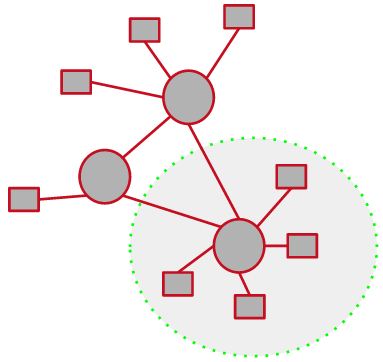
\includegraphics[width=0.4\textwidth]{graphics/hostgroup.png}
    \caption{HostGroup in network topology}
    \label{fig:hostgroup}
\end{figure}

First, we define a Host Group. A network device (circle in Figure \ref{fig:hostgroup}) and all
directly connected hosts (rectangles on the Figure \ref{fig:hostgroup}) constitute a Host Group.
Thus, network topology consists of a set of Host Groups and each of them consists of one switch and
a set of hosts. Furthermore, we define the quality of the link between the hosts by affiliation of
the hosts to the same Host Group.

\begin{equation}
    weight\_full = data\_size / (bandwidth - bandwidth\_used) + latency
\end{equation}
\begin{equation}
    weight'_simple = data\_size / bandwidth
\end{equation}

If two hosts are not in the same Host Group, the quality of the connection between them is the
transmission time for the data needed to be sent between the switches of the two Host Groups where
the hosts belong to. This value weight of the edge in the topology graph is used to calculate the
shortest paths by the Dijkstra algorithm. In case there are no statistics about current utilization
of the network, a default size can be applied.\\

\begin{lstlisting}[caption=Algorithm of finding free hosts based on Host Group concept]
IP: findNextBestHost()
    if no_free_hosts()
        return NULL
    if all_hosts_are_free()
        return get_biggest_host_group().getFreeHost()
    if working_host_group_has_free_hosts()
        return free_host_group.getFreeHost()
    else
        return next_best_host_group().getFreeHost()
end
\end{lstlisting}

The algorithm in pseudocode is shown in the Listing 1. Basically, there are only four options. If
there are no free hosts available, the data process engine will not get any host for its
calculations. In case that all hosts are free, the biggest Host Group will be selected and the data
processing engine receives one of the host for executions. If there is a Host Group with some
occupied and idle hosts, one idle host will be returned to the data processing engine. In the last
case, there are some Host Groups which are fully occupied. In order to find the next best Host
Group, the algorithm searches for the Host Group with the best link to the Host Groups that is
currently occupied using shortest paths calculated by Dijkstras’ algorithm.

The implementation of this concept and algorithms is thread safe and optimized to be efficient
(caching). Furthermore, the algorithms can be easily adapted to execute different parallel jobs on
the same topology at the same time.

\subsection{Future Work}
\subsubsection{Traffic Properties}
Monitoring would be an enabler for better scheduling and flow programming, by taking latency and
network utilization into account.

The OpenFlow specification \cite{openflow} offers port- and flow-based packet- and byte-counters,
but neither is measures latency nor bandwidth. Therefore monitoring has to be somehow implemented.
One approach to determine latency between two switches is to insert additional packets and measure
the duration. The PACKET OUT and PACKET IN functions of OpenFlow would be used. PACKET OUT messages
forward additional packages to one or more ports. The payload of this message is the timestamp of
its creation. The OpenFlow controller receives a PACKET IN message when a switch could not assign a
packet to a flow of its flow table. The latency can then be easily calculated by subtracting the
time of packet creation and roundtrip times from the time the packet was received via PACKET IN. The
roundtrip times can be measured by sending a packet to a switch, which is returned immediately.
\cite{monitoringlatency} \cite{opennetmon}

OpenFlow also supports a FLOW REMOVED message that is received by the controller when a flow entry
of a switch is expired since every flow entry exists only for a certain period of time. This message
contains information about the duration an entry was active in the flow table, the amount of traffic
matched against an entry and the input port to determine the source of traffic. These information
enable the computation of utilization between inter-switch links. This approach does not produce any
instrumentation overhead since the FLOW REMOVED messages are send anyhow. A drawback might be that
the information are only available for the point of time when the flow was removed. \cite{flowsense}

Another way to measure network utilization is to poll the OpenFlow statistics. Fetching the
statistics of a switch causes some overhead, therefore the problem is to find an intelligent polling
algorithm to reduce the load on switches. Using the routing information of a flow is helpful to find
an appropriate querying strategy. The switch closest to the destination offers the most accurate
statistics but there would be a huge load on this switch. While querying a switch randomly has
better load balancing but is less accurate. A good compromise is to query two switches randomly and
select the one closer to the destination. \cite{opentm} \cite{opennetmon}

There are implementations for the OpenFlow Controller POX \cite{opennetmon}, NOX \cite{opentm} and
Floodlight \cite {flowsense}.

\subsubsection{Loadbalancing}
Even using the Bottom Up approach, the possibility to control data flows in the network still
remains. The notion of balancing data flows of alike source and sink around multiple paths comes to
mind. OpenDaylights’ default flow configuration behavior is handled by an interchangeable part
application titled Simple Forwarding. Upon activation by a switch clueless how to reach a packets’
destination, the application prompts the updating of all switches connected to the controller so
that future packets to the said destination host will follow along the shortest path. This behavior
might be sufficient in the case where sources and sinks are not grouped around common switches but
in our case we would have lots of tasks deployed on host groups characterized by single switch
connections due to our scheduling decisions. In the assumed case of all-to-all data-flows between
two or more host groups, we would not want to send all data along a single path. Even with the
switch of each host group posing as a natural bottleneck, we assume better overall load balancing
would stem from using more than a single shortest path which we could determine with Yen’s
Algorithm.
